\documentclass{book}
\usepackage{CJKutf8}
\usepackage{amsmath}
\usepackage{amsfonts}
\usepackage{amsthm}
\usepackage{titlesec}
\usepackage{titletoc}
\usepackage{xCJKnumb}
\usepackage{tikz}
\begin{document}
\begin{CJK*}{UTF8}{gbsn}
  \title{离散数学}
  \author{陈建文}
  \maketitle

  \titleformat{\chapter}{\centering\Huge\bfseries}{第\, \xCJKnumber{\thechapter}\,
    章}{1em}{}
%  \renewcommand{\chaptermark}[1]{\markboth{第 \thechapter 章}{}}
  \newtheorem{Ex}{习题}[chapter]

  

  \chapter{集合}
\begin{Ex}[课本第8页第3题]
  \mbox{} \par \noindent
  
写出方程
\begin{equation*}
x^2+2x+1=0
\end{equation*}
的根构成的集合。
\end{Ex}
\begin{proof}[证明]
$\{-1\}$
\end{proof}

  \chapter{映射}
\begin{Ex}
设$f$是从实数集合$\mathbb{R}$到实数集合$\mathbb{R}$的映射,$f(x) = x^2$,
$A=\{-1,0\}$, $B=\{0,1\}$,$f(A \cap B)=\underline{\quad\quad}$, $f(A) \cap
f(B) = \underline{\quad\quad}$。
\end{Ex}

\begin{Ex}
设$f$是从集合$A$到集合$B$的映射,求证$f(A \cap B) \subseteq f(A) \cap f(B)$。
\end{Ex}

  \chapter{置换}
\begin{Ex}
  设$S(n,k)$表示$S_n$中的恰有$k$个循环的(包括$1-$循环)的置换的个数。证明:
  \[\sum_{k=1}^nS(n,k)x^k = x(x+1)(x+2)\cdots(x+n-1)\]
\end{Ex}

  \chapter{欧拉图}
\begin{Ex}
  以下4个图中,存在欧拉闭迹的是$\underline{\quad\quad}$。
  \vspace{0.5cm}

  A.
    \begin{minipage}{0.18\linewidth}
    \centering
    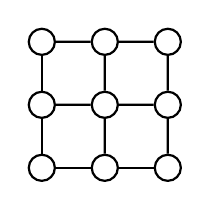
\begin{tikzpicture}[auto,
    specification/.style ={circle, draw, thick}, scale = 0.8]
   \node[specification] (A)  at (0,0)  {};
   \node[specification] (B)  at (1,0)  {};
   \node[specification] (C)  at (2,0)  {};
   \node[specification] (D)  at (0,1)  {};
   \node[specification] (E)  at (1,1)  {};
   \node[specification] (F)  at (2,1)  {};
   \node[specification] (G)  at (0,2)  {};
   \node[specification] (H)  at (1,2)  {};
   \node[specification] (I)  at (2,2)  {};

   \draw[thick] (A) to  (B);
   \draw[thick] (B) to  (C);
   \draw[thick] (D) to  (E);
   \draw[thick] (E) to  (F);
   \draw[thick] (G) to (H);
   \draw[thick] (H) to (I);
   \draw[thick] (A) to (D);
   \draw[thick] (B) to (E);
   \draw[thick] (C) to (F);
   \draw[thick] (D) to (G);
   \draw[thick] (E) to (H);
   \draw[thick] (F) to (I);
 \end{tikzpicture}
\end{minipage}\hfill
  B.
    \begin{minipage}{0.18\linewidth}
    \centering
    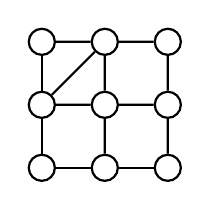
\begin{tikzpicture}[auto,
    specification/.style ={circle, draw, thick}, scale = 0.8]
   \node[specification] (A)  at (0,0)  {};
   \node[specification] (B)  at (1,0)  {};
   \node[specification] (C)  at (2,0)  {};
   \node[specification] (D)  at (0,1)  {};
   \node[specification] (E)  at (1,1)  {};
   \node[specification] (F)  at (2,1)  {};
   \node[specification] (G)  at (0,2)  {};
   \node[specification] (H)  at (1,2)  {};
   \node[specification] (I)  at (2,2)  {};

   \draw[thick] (A) to  (B);
   \draw[thick] (B) to  (C);
   \draw[thick] (D) to  (E);
   \draw[thick] (E) to  (F);
   \draw[thick] (G) to (H);
   \draw[thick] (H) to (I);
   \draw[thick] (A) to (D);
   \draw[thick] (B) to (E);
   \draw[thick] (C) to (F);
   \draw[thick] (D) to (G);
   \draw[thick] (E) to (H);
   \draw[thick] (F) to (I);
   \draw[thick] (D) to (H);

 \end{tikzpicture}
\end{minipage}\hfill
      C.
    \begin{minipage}{0.18\linewidth}
    \centering
    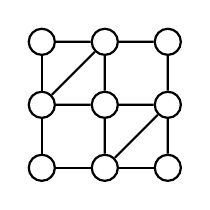
\begin{tikzpicture}[auto,
    specification/.style ={circle, draw, thick}, scale=0.8]
   \node[specification] (A)  at (0,0)  {};
   \node[specification] (B)  at (1,0)  {};
   \node[specification] (C)  at (2,0)  {};
   \node[specification] (D)  at (0,1)  {};
   \node[specification] (E)  at (1,1)  {};
   \node[specification] (F)  at (2,1)  {};
   \node[specification] (G)  at (0,2)  {};
   \node[specification] (H)  at (1,2)  {};
   \node[specification] (I)  at (2,2)  {};

   \draw[thick] (A) to  (B);
   \draw[thick] (B) to  (C);
   \draw[thick] (D) to  (E);
   \draw[thick] (E) to  (F);
   \draw[thick] (G) to (H);
   \draw[thick] (H) to (I);
   \draw[thick] (A) to (D);
   \draw[thick] (B) to (E);
   \draw[thick] (C) to (F);
   \draw[thick] (D) to (G);
   \draw[thick] (E) to (H);
   \draw[thick] (F) to (I);
   \draw[thick] (D) to (H);
   \draw[thick] (B) to (F);
 \end{tikzpicture}
\end{minipage}\hfill
      D.
    \begin{minipage}{0.18\linewidth}
    \centering
    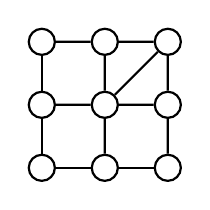
\begin{tikzpicture}[auto,
    specification/.style ={circle, draw, thick}, scale=0.8]
   \node[specification] (A)  at (0,0)  {};
   \node[specification] (B)  at (1,0)  {};
   \node[specification] (C)  at (2,0)  {};
   \node[specification] (D)  at (0,1)  {};
   \node[specification] (E)  at (1,1)  {};
   \node[specification] (F)  at (2,1)  {};
   \node[specification] (G)  at (0,2)  {};
   \node[specification] (H)  at (1,2)  {};
   \node[specification] (I)  at (2,2)  {};

   \draw[thick] (A) to  (B);
   \draw[thick] (B) to  (C);
   \draw[thick] (D) to  (E);
   \draw[thick] (E) to  (F);
   \draw[thick] (G) to (H);
   \draw[thick] (H) to (I);
   \draw[thick] (A) to (D);
   \draw[thick] (B) to (E);
   \draw[thick] (C) to (F);
   \draw[thick] (D) to (G);
   \draw[thick] (E) to (H);
   \draw[thick] (F) to (I);
   \draw[thick] (E) to (I);

 \end{tikzpicture}
\end{minipage}\hfill

\end{Ex}

\begin{Ex}
  以下4个图中,存在一条欧拉开迹的是$\underline{\quad\quad}$。
  \vspace{0.5cm}

  A.
    \begin{minipage}{0.18\linewidth}
    \centering
    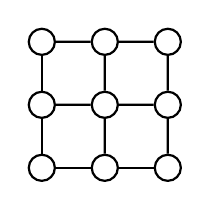
\begin{tikzpicture}[auto,
    specification/.style ={circle, draw, thick}, scale = 0.8]
   \node[specification] (A)  at (0,0)  {};
   \node[specification] (B)  at (1,0)  {};
   \node[specification] (C)  at (2,0)  {};
   \node[specification] (D)  at (0,1)  {};
   \node[specification] (E)  at (1,1)  {};
   \node[specification] (F)  at (2,1)  {};
   \node[specification] (G)  at (0,2)  {};
   \node[specification] (H)  at (1,2)  {};
   \node[specification] (I)  at (2,2)  {};

   \draw[thick] (A) to  (B);
   \draw[thick] (B) to  (C);
   \draw[thick] (D) to  (E);
   \draw[thick] (E) to  (F);
   \draw[thick] (G) to (H);
   \draw[thick] (H) to (I);
   \draw[thick] (A) to (D);
   \draw[thick] (B) to (E);
   \draw[thick] (C) to (F);
   \draw[thick] (D) to (G);
   \draw[thick] (E) to (H);
   \draw[thick] (F) to (I);
 \end{tikzpicture}
\end{minipage}\hfill
  B.
    \begin{minipage}{0.18\linewidth}
    \centering
    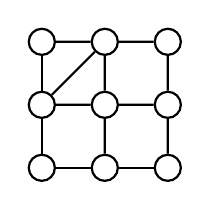
\begin{tikzpicture}[auto,
    specification/.style ={circle, draw, thick}, scale = 0.8]
   \node[specification] (A)  at (0,0)  {};
   \node[specification] (B)  at (1,0)  {};
   \node[specification] (C)  at (2,0)  {};
   \node[specification] (D)  at (0,1)  {};
   \node[specification] (E)  at (1,1)  {};
   \node[specification] (F)  at (2,1)  {};
   \node[specification] (G)  at (0,2)  {};
   \node[specification] (H)  at (1,2)  {};
   \node[specification] (I)  at (2,2)  {};

   \draw[thick] (A) to  (B);
   \draw[thick] (B) to  (C);
   \draw[thick] (D) to  (E);
   \draw[thick] (E) to  (F);
   \draw[thick] (G) to (H);
   \draw[thick] (H) to (I);
   \draw[thick] (A) to (D);
   \draw[thick] (B) to (E);
   \draw[thick] (C) to (F);
   \draw[thick] (D) to (G);
   \draw[thick] (E) to (H);
   \draw[thick] (F) to (I);
   \draw[thick] (D) to (H);

 \end{tikzpicture}
\end{minipage}\hfill
      C.
    \begin{minipage}{0.18\linewidth}
    \centering
    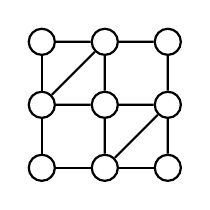
\begin{tikzpicture}[auto,
    specification/.style ={circle, draw, thick}, scale=0.8]
   \node[specification] (A)  at (0,0)  {};
   \node[specification] (B)  at (1,0)  {};
   \node[specification] (C)  at (2,0)  {};
   \node[specification] (D)  at (0,1)  {};
   \node[specification] (E)  at (1,1)  {};
   \node[specification] (F)  at (2,1)  {};
   \node[specification] (G)  at (0,2)  {};
   \node[specification] (H)  at (1,2)  {};
   \node[specification] (I)  at (2,2)  {};

   \draw[thick] (A) to  (B);
   \draw[thick] (B) to  (C);
   \draw[thick] (D) to  (E);
   \draw[thick] (E) to  (F);
   \draw[thick] (G) to (H);
   \draw[thick] (H) to (I);
   \draw[thick] (A) to (D);
   \draw[thick] (B) to (E);
   \draw[thick] (C) to (F);
   \draw[thick] (D) to (G);
   \draw[thick] (E) to (H);
   \draw[thick] (F) to (I);
   \draw[thick] (D) to (H);
   \draw[thick] (B) to (F);
 \end{tikzpicture}
\end{minipage}\hfill
      D.
    \begin{minipage}{0.18\linewidth}
    \centering
    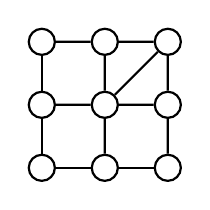
\begin{tikzpicture}[auto,
    specification/.style ={circle, draw, thick}, scale=0.8]
   \node[specification] (A)  at (0,0)  {};
   \node[specification] (B)  at (1,0)  {};
   \node[specification] (C)  at (2,0)  {};
   \node[specification] (D)  at (0,1)  {};
   \node[specification] (E)  at (1,1)  {};
   \node[specification] (F)  at (2,1)  {};
   \node[specification] (G)  at (0,2)  {};
   \node[specification] (H)  at (1,2)  {};
   \node[specification] (I)  at (2,2)  {};

   \draw[thick] (A) to  (B);
   \draw[thick] (B) to  (C);
   \draw[thick] (D) to  (E);
   \draw[thick] (E) to  (F);
   \draw[thick] (G) to (H);
   \draw[thick] (H) to (I);
   \draw[thick] (A) to (D);
   \draw[thick] (B) to (E);
   \draw[thick] (C) to (F);
   \draw[thick] (D) to (G);
   \draw[thick] (E) to (H);
   \draw[thick] (F) to (I);
   \draw[thick] (E) to (I);

 \end{tikzpicture}
\end{minipage}\hfill

\end{Ex}

\begin{Ex}
  以下4个图中,不可以一笔画成的是$\underline{\quad\quad}$。
  \vspace{0.5cm}

  A.
    \begin{minipage}{0.18\linewidth}
    \centering
    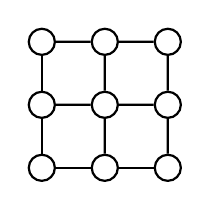
\begin{tikzpicture}[auto,
    specification/.style ={circle, draw, thick}, scale = 0.8]
   \node[specification] (A)  at (0,0)  {};
   \node[specification] (B)  at (1,0)  {};
   \node[specification] (C)  at (2,0)  {};
   \node[specification] (D)  at (0,1)  {};
   \node[specification] (E)  at (1,1)  {};
   \node[specification] (F)  at (2,1)  {};
   \node[specification] (G)  at (0,2)  {};
   \node[specification] (H)  at (1,2)  {};
   \node[specification] (I)  at (2,2)  {};

   \draw[thick] (A) to  (B);
   \draw[thick] (B) to  (C);
   \draw[thick] (D) to  (E);
   \draw[thick] (E) to  (F);
   \draw[thick] (G) to (H);
   \draw[thick] (H) to (I);
   \draw[thick] (A) to (D);
   \draw[thick] (B) to (E);
   \draw[thick] (C) to (F);
   \draw[thick] (D) to (G);
   \draw[thick] (E) to (H);
   \draw[thick] (F) to (I);
 \end{tikzpicture}
\end{minipage}\hfill
  B.
    \begin{minipage}{0.18\linewidth}
    \centering
    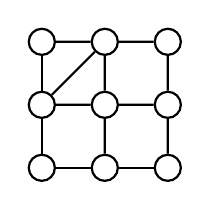
\begin{tikzpicture}[auto,
    specification/.style ={circle, draw, thick}, scale = 0.8]
   \node[specification] (A)  at (0,0)  {};
   \node[specification] (B)  at (1,0)  {};
   \node[specification] (C)  at (2,0)  {};
   \node[specification] (D)  at (0,1)  {};
   \node[specification] (E)  at (1,1)  {};
   \node[specification] (F)  at (2,1)  {};
   \node[specification] (G)  at (0,2)  {};
   \node[specification] (H)  at (1,2)  {};
   \node[specification] (I)  at (2,2)  {};

   \draw[thick] (A) to  (B);
   \draw[thick] (B) to  (C);
   \draw[thick] (D) to  (E);
   \draw[thick] (E) to  (F);
   \draw[thick] (G) to (H);
   \draw[thick] (H) to (I);
   \draw[thick] (A) to (D);
   \draw[thick] (B) to (E);
   \draw[thick] (C) to (F);
   \draw[thick] (D) to (G);
   \draw[thick] (E) to (H);
   \draw[thick] (F) to (I);
   \draw[thick] (D) to (H);

 \end{tikzpicture}
\end{minipage}\hfill
      C.
    \begin{minipage}{0.18\linewidth}
    \centering
    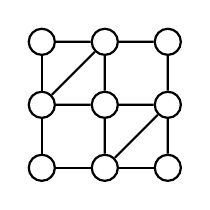
\begin{tikzpicture}[auto,
    specification/.style ={circle, draw, thick}, scale=0.8]
   \node[specification] (A)  at (0,0)  {};
   \node[specification] (B)  at (1,0)  {};
   \node[specification] (C)  at (2,0)  {};
   \node[specification] (D)  at (0,1)  {};
   \node[specification] (E)  at (1,1)  {};
   \node[specification] (F)  at (2,1)  {};
   \node[specification] (G)  at (0,2)  {};
   \node[specification] (H)  at (1,2)  {};
   \node[specification] (I)  at (2,2)  {};

   \draw[thick] (A) to  (B);
   \draw[thick] (B) to  (C);
   \draw[thick] (D) to  (E);
   \draw[thick] (E) to  (F);
   \draw[thick] (G) to (H);
   \draw[thick] (H) to (I);
   \draw[thick] (A) to (D);
   \draw[thick] (B) to (E);
   \draw[thick] (C) to (F);
   \draw[thick] (D) to (G);
   \draw[thick] (E) to (H);
   \draw[thick] (F) to (I);
   \draw[thick] (D) to (H);
   \draw[thick] (B) to (F);
 \end{tikzpicture}
\end{minipage}\hfill
      D.
    \begin{minipage}{0.18\linewidth}
    \centering
    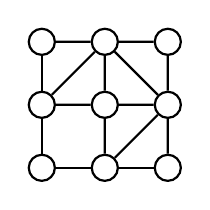
\begin{tikzpicture}[auto,
    specification/.style ={circle, draw, thick}, scale=0.8]
   \node[specification] (A)  at (0,0)  {};
   \node[specification] (B)  at (1,0)  {};
   \node[specification] (C)  at (2,0)  {};
   \node[specification] (D)  at (0,1)  {};
   \node[specification] (E)  at (1,1)  {};
   \node[specification] (F)  at (2,1)  {};
   \node[specification] (G)  at (0,2)  {};
   \node[specification] (H)  at (1,2)  {};
   \node[specification] (I)  at (2,2)  {};

   \draw[thick] (A) to  (B);
   \draw[thick] (B) to  (C);
   \draw[thick] (D) to  (E);
   \draw[thick] (E) to  (F);
   \draw[thick] (G) to (H);
   \draw[thick] (H) to (I);
   \draw[thick] (A) to (D);
   \draw[thick] (B) to (E);
   \draw[thick] (C) to (F);
   \draw[thick] (D) to (G);
   \draw[thick] (E) to (H);
   \draw[thick] (F) to (I);
   \draw[thick] (D) to (H);
   \draw[thick] (B) to (F);
   \draw[thick] (H) to (F);

 \end{tikzpicture}
\end{minipage}\hfill


\end{Ex}


\begin{Ex}
  以下4个图中,至少需要两笔才能画成的是$\underline{\quad\quad}$。
  \vspace{0.5cm}

  A.
    \begin{minipage}{0.18\linewidth}
    \centering
    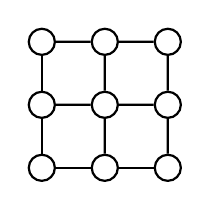
\begin{tikzpicture}[auto,
    specification/.style ={circle, draw, thick}, scale = 0.8]
   \node[specification] (A)  at (0,0)  {};
   \node[specification] (B)  at (1,0)  {};
   \node[specification] (C)  at (2,0)  {};
   \node[specification] (D)  at (0,1)  {};
   \node[specification] (E)  at (1,1)  {};
   \node[specification] (F)  at (2,1)  {};
   \node[specification] (G)  at (0,2)  {};
   \node[specification] (H)  at (1,2)  {};
   \node[specification] (I)  at (2,2)  {};

   \draw[thick] (A) to  (B);
   \draw[thick] (B) to  (C);
   \draw[thick] (D) to  (E);
   \draw[thick] (E) to  (F);
   \draw[thick] (G) to (H);
   \draw[thick] (H) to (I);
   \draw[thick] (A) to (D);
   \draw[thick] (B) to (E);
   \draw[thick] (C) to (F);
   \draw[thick] (D) to (G);
   \draw[thick] (E) to (H);
   \draw[thick] (F) to (I);
 \end{tikzpicture}
\end{minipage}\hfill
  B.
    \begin{minipage}{0.18\linewidth}
    \centering
    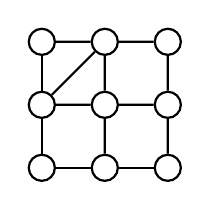
\begin{tikzpicture}[auto,
    specification/.style ={circle, draw, thick}, scale = 0.8]
   \node[specification] (A)  at (0,0)  {};
   \node[specification] (B)  at (1,0)  {};
   \node[specification] (C)  at (2,0)  {};
   \node[specification] (D)  at (0,1)  {};
   \node[specification] (E)  at (1,1)  {};
   \node[specification] (F)  at (2,1)  {};
   \node[specification] (G)  at (0,2)  {};
   \node[specification] (H)  at (1,2)  {};
   \node[specification] (I)  at (2,2)  {};

   \draw[thick] (A) to  (B);
   \draw[thick] (B) to  (C);
   \draw[thick] (D) to  (E);
   \draw[thick] (E) to  (F);
   \draw[thick] (G) to (H);
   \draw[thick] (H) to (I);
   \draw[thick] (A) to (D);
   \draw[thick] (B) to (E);
   \draw[thick] (C) to (F);
   \draw[thick] (D) to (G);
   \draw[thick] (E) to (H);
   \draw[thick] (F) to (I);
   \draw[thick] (D) to (H);

 \end{tikzpicture}
\end{minipage}\hfill
      C.
    \begin{minipage}{0.18\linewidth}
    \centering
    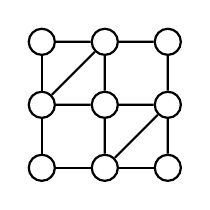
\begin{tikzpicture}[auto,
    specification/.style ={circle, draw, thick}, scale=0.8]
   \node[specification] (A)  at (0,0)  {};
   \node[specification] (B)  at (1,0)  {};
   \node[specification] (C)  at (2,0)  {};
   \node[specification] (D)  at (0,1)  {};
   \node[specification] (E)  at (1,1)  {};
   \node[specification] (F)  at (2,1)  {};
   \node[specification] (G)  at (0,2)  {};
   \node[specification] (H)  at (1,2)  {};
   \node[specification] (I)  at (2,2)  {};

   \draw[thick] (A) to  (B);
   \draw[thick] (B) to  (C);
   \draw[thick] (D) to  (E);
   \draw[thick] (E) to  (F);
   \draw[thick] (G) to (H);
   \draw[thick] (H) to (I);
   \draw[thick] (A) to (D);
   \draw[thick] (B) to (E);
   \draw[thick] (C) to (F);
   \draw[thick] (D) to (G);
   \draw[thick] (E) to (H);
   \draw[thick] (F) to (I);
   \draw[thick] (D) to (H);
   \draw[thick] (B) to (F);
 \end{tikzpicture}
\end{minipage}\hfill
      D.
    \begin{minipage}{0.18\linewidth}
    \centering
    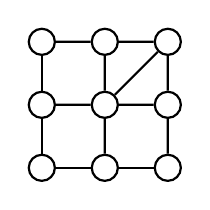
\begin{tikzpicture}[auto,
    specification/.style ={circle, draw, thick}, scale=0.8]
   \node[specification] (A)  at (0,0)  {};
   \node[specification] (B)  at (1,0)  {};
   \node[specification] (C)  at (2,0)  {};
   \node[specification] (D)  at (0,1)  {};
   \node[specification] (E)  at (1,1)  {};
   \node[specification] (F)  at (2,1)  {};
   \node[specification] (G)  at (0,2)  {};
   \node[specification] (H)  at (1,2)  {};
   \node[specification] (I)  at (2,2)  {};

   \draw[thick] (A) to  (B);
   \draw[thick] (B) to  (C);
   \draw[thick] (D) to  (E);
   \draw[thick] (E) to  (F);
   \draw[thick] (G) to (H);
   \draw[thick] (H) to (I);
   \draw[thick] (A) to (D);
   \draw[thick] (B) to (E);
   \draw[thick] (C) to (F);
   \draw[thick] (D) to (G);
   \draw[thick] (E) to (H);
   \draw[thick] (F) to (I);
   \draw[thick] (E) to (I);

 \end{tikzpicture}
\end{minipage}\hfill

\end{Ex}


\begin{Ex}
  以下4个图中,至少需要三笔才能画成的是$\underline{\quad\quad}$。
  \vspace{0.5cm}

  A.
    \begin{minipage}{0.18\linewidth}
    \centering
    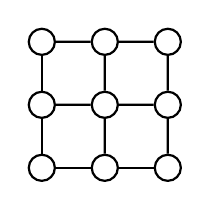
\begin{tikzpicture}[auto,
    specification/.style ={circle, draw, thick}, scale = 0.8]
   \node[specification] (A)  at (0,0)  {};
   \node[specification] (B)  at (1,0)  {};
   \node[specification] (C)  at (2,0)  {};
   \node[specification] (D)  at (0,1)  {};
   \node[specification] (E)  at (1,1)  {};
   \node[specification] (F)  at (2,1)  {};
   \node[specification] (G)  at (0,2)  {};
   \node[specification] (H)  at (1,2)  {};
   \node[specification] (I)  at (2,2)  {};

   \draw[thick] (A) to  (B);
   \draw[thick] (B) to  (C);
   \draw[thick] (D) to  (E);
   \draw[thick] (E) to  (F);
   \draw[thick] (G) to (H);
   \draw[thick] (H) to (I);
   \draw[thick] (A) to (D);
   \draw[thick] (B) to (E);
   \draw[thick] (C) to (F);
   \draw[thick] (D) to (G);
   \draw[thick] (E) to (H);
   \draw[thick] (F) to (I);
 \end{tikzpicture}
\end{minipage}\hfill
  B.
    \begin{minipage}{0.18\linewidth}
    \centering
    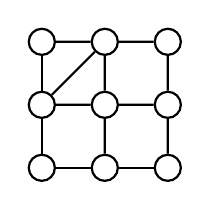
\begin{tikzpicture}[auto,
    specification/.style ={circle, draw, thick}, scale = 0.8]
   \node[specification] (A)  at (0,0)  {};
   \node[specification] (B)  at (1,0)  {};
   \node[specification] (C)  at (2,0)  {};
   \node[specification] (D)  at (0,1)  {};
   \node[specification] (E)  at (1,1)  {};
   \node[specification] (F)  at (2,1)  {};
   \node[specification] (G)  at (0,2)  {};
   \node[specification] (H)  at (1,2)  {};
   \node[specification] (I)  at (2,2)  {};

   \draw[thick] (A) to  (B);
   \draw[thick] (B) to  (C);
   \draw[thick] (D) to  (E);
   \draw[thick] (E) to  (F);
   \draw[thick] (G) to (H);
   \draw[thick] (H) to (I);
   \draw[thick] (A) to (D);
   \draw[thick] (B) to (E);
   \draw[thick] (C) to (F);
   \draw[thick] (D) to (G);
   \draw[thick] (E) to (H);
   \draw[thick] (F) to (I);
   \draw[thick] (D) to (H);

 \end{tikzpicture}
\end{minipage}\hfill
      C.
    \begin{minipage}{0.18\linewidth}
    \centering
    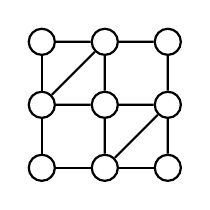
\begin{tikzpicture}[auto,
    specification/.style ={circle, draw, thick}, scale=0.8]
   \node[specification] (A)  at (0,0)  {};
   \node[specification] (B)  at (1,0)  {};
   \node[specification] (C)  at (2,0)  {};
   \node[specification] (D)  at (0,1)  {};
   \node[specification] (E)  at (1,1)  {};
   \node[specification] (F)  at (2,1)  {};
   \node[specification] (G)  at (0,2)  {};
   \node[specification] (H)  at (1,2)  {};
   \node[specification] (I)  at (2,2)  {};

   \draw[thick] (A) to  (B);
   \draw[thick] (B) to  (C);
   \draw[thick] (D) to  (E);
   \draw[thick] (E) to  (F);
   \draw[thick] (G) to (H);
   \draw[thick] (H) to (I);
   \draw[thick] (A) to (D);
   \draw[thick] (B) to (E);
   \draw[thick] (C) to (F);
   \draw[thick] (D) to (G);
   \draw[thick] (E) to (H);
   \draw[thick] (F) to (I);
   \draw[thick] (D) to (H);
   \draw[thick] (B) to (F);
 \end{tikzpicture}
\end{minipage}\hfill
      D.
    \begin{minipage}{0.18\linewidth}
    \centering
    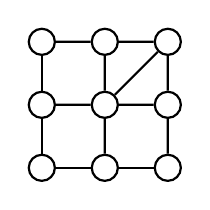
\begin{tikzpicture}[auto,
    specification/.style ={circle, draw, thick}, scale=0.8]
   \node[specification] (A)  at (0,0)  {};
   \node[specification] (B)  at (1,0)  {};
   \node[specification] (C)  at (2,0)  {};
   \node[specification] (D)  at (0,1)  {};
   \node[specification] (E)  at (1,1)  {};
   \node[specification] (F)  at (2,1)  {};
   \node[specification] (G)  at (0,2)  {};
   \node[specification] (H)  at (1,2)  {};
   \node[specification] (I)  at (2,2)  {};

   \draw[thick] (A) to  (B);
   \draw[thick] (B) to  (C);
   \draw[thick] (D) to  (E);
   \draw[thick] (E) to  (F);
   \draw[thick] (G) to (H);
   \draw[thick] (H) to (I);
   \draw[thick] (A) to (D);
   \draw[thick] (B) to (E);
   \draw[thick] (C) to (F);
   \draw[thick] (D) to (G);
   \draw[thick] (E) to (H);
   \draw[thick] (F) to (I);
   \draw[thick] (E) to (I);

 \end{tikzpicture}
\end{minipage}\hfill

\end{Ex}

  \chapter{综合题}

\begin{Ex}
  给出以下四个图的顶点最小度、顶点连通度、边连通度、色数,并说明它们是否为连通图、
  偶图、欧拉图、哈
  密顿图、可平面图。
  
\vspace{0.5cm}
    \begin{minipage}{0.49\linewidth}
    \centering
    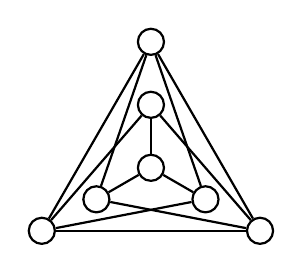
\begin{tikzpicture}[auto,
    specification/.style ={circle, draw, thick}, scale = 0.8]
   \node[specification] (A)  at (0,0)  {};
   \node[specification] (B)  at (90:2cm)  {};
   \node[specification] (C)  at (210:2cm)  {};
   \node[specification] (D)  at (330:2cm)  {};
   \node[specification] (E)  at (90:1cm)  {};
   \node[specification] (F)  at (210:1cm)  {};
   \node[specification] (G)  at (330:1cm)  {};


   \draw[thick] (B) to  (C);
   \draw[thick] (C) to  (D);
   \draw[thick] (D) to  (B);
   
   
   \draw[thick] (E) to (C);
   \draw[thick] (E) to (D);

   \draw[thick] (A) to (E);
   \draw[thick] (A) to (F);
   \draw[thick] (A) to (G);

   \draw[thick] (B) to (F);
   \draw[thick] (B) to (G);

   \draw[thick] (C) to (G);
   \draw[thick] (D) to (F);

      


   
 \end{tikzpicture}

 (a)
\end{minipage}\hfill
    \begin{minipage}{0.49\linewidth}
    \centering
    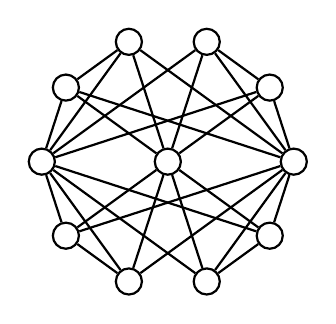
\begin{tikzpicture}[auto,
    specification/.style ={circle, draw, thick}, scale = 0.8]
   \node[specification] (A)  at (0:2cm)  {};
   \node[specification] (B)  at (36:2cm)  {};
   \node[specification] (C)  at (2*36:2cm)  {};
   \node[specification] (D)  at (3*36:2cm)  {};
   \node[specification] (E)  at (4*36:2cm)  {};
   \node[specification] (F)  at (5*36:2cm)  {};
   \node[specification] (G)  at (6*36:2cm)  {};
   \node[specification] (H)  at (7*36:2cm)  {};
   \node[specification] (I)  at (8*36:2cm)  {};
   \node[specification] (J)  at (9*36:2cm)  {};
   \node[specification] (O)  at (0,0)  {};

   \draw[thick] (O) to  (B);
   \draw[thick] (O) to  (C);
   \draw[thick] (O) to  (D);
   \draw[thick] (O) to  (E);
   \draw[thick] (O) to  (G);
   \draw[thick] (O) to  (H);
   \draw[thick] (O) to  (I);
   \draw[thick] (O) to  (J);

   \draw[thick] (A) to  (B);
   \draw[thick] (B) to  (C);
   \draw[thick] (A) to  (J);
   \draw[thick] (J) to  (I);

   \draw[thick] (D) to  (E);
   \draw[thick] (E) to  (F);
   \draw[thick] (F) to  (G);
   \draw[thick] (G) to  (H);

   \draw[thick] (A) to  (C);
   \draw[thick] (A) to  (D);
   \draw[thick] (A) to  (E);
   \draw[thick] (A) to  (G);
   \draw[thick] (A) to  (H);
   \draw[thick] (A) to  (I);


   \draw[thick] (F) to  (B);
   \draw[thick] (F) to  (C);
   \draw[thick] (F) to  (D);
   \draw[thick] (F) to  (H);
   \draw[thick] (F) to  (I);
   \draw[thick] (F) to  (J);
 \end{tikzpicture}

 (b)
\end{minipage}


    \begin{minipage}{0.49\linewidth}
    \centering
    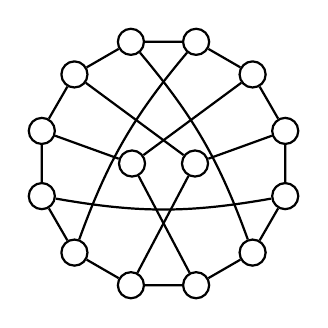
\begin{tikzpicture}[auto,
      specification/.style ={circle, draw, thick}, scale=0.8]

   \node[specification] (A)  at (15:2cm)  {};
   \node[specification] (B)  at (15+30:2cm)  {};
   \node[specification] (C)  at (15+2*30:2cm)  {};
   \node[specification] (D)  at (15+3*30:2cm)  {};
   \node[specification] (E)  at (15+4*30:2cm)  {};
   \node[specification] (F)  at (15+5*30:2cm)  {};
   \node[specification] (G)  at (15+6*30:2cm)  {};
   \node[specification] (H)  at (15+7*30:2cm)  {};
   \node[specification] (I)  at (15+8*30:2cm)  {};
   \node[specification] (J)  at (15+9*30:2cm)  {};
   \node[specification] (K)  at (15+10*30:2cm)  {};
   \node[specification] (L)  at (15+11*30:2cm)  {};
   \node[specification] (X)  at (-0.5cm, 0cm)  {};
   \node[specification] (Y)  at (0.5cm, 0cm)  {};
   
   


   \draw[thick] (A) to  (B);
   \draw[thick] (B) to  (C);
   \draw[thick] (C) to  (D);
   \draw[thick] (D) to  (E);
   \draw[thick] (E) to  (F);
   \draw[thick] (F) to  (G);
   \draw[thick] (G) to (H);
   \draw[thick] (H) to (I);
   \draw[thick] (I) to  (J);
   \draw[thick] (J) to  (K);
   \draw[thick] (K) to  (L);
   \draw[thick] (L) to  (A);

   \draw[thick] (C) to [bend right = 10] (H);
   \draw[thick] (D) to [bend left = 10] (K);
   \draw[thick] (G) to [bend right = 10] (L);

   \draw[thick] (X) to  (B);
   \draw[thick] (X) to  (F);
   \draw[thick] (X) to  (J);

   \draw[thick] (Y) to  (A);
   \draw[thick] (Y) to  (E);
   \draw[thick] (Y) to  (I);



   

 \end{tikzpicture}

 (c)
\end{minipage}\hfill
    \begin{minipage}{0.49\linewidth}
    \centering
    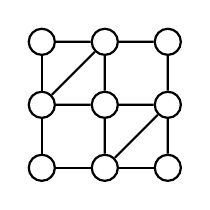
\begin{tikzpicture}[auto,
    specification/.style ={circle, draw, thick}, scale=0.8]
   \node[specification] (A)  at (0,0)  {};
   \node[specification] (B)  at (1,0)  {};
   \node[specification] (C)  at (2,0)  {};
   \node[specification] (D)  at (0,1)  {};
   \node[specification] (E)  at (1,1)  {};
   \node[specification] (F)  at (2,1)  {};
   \node[specification] (G)  at (0,2)  {};
   \node[specification] (H)  at (1,2)  {};
   \node[specification] (I)  at (2,2)  {};

   \draw[thick] (A) to  (B);
   \draw[thick] (B) to  (C);
   \draw[thick] (D) to  (E);
   \draw[thick] (E) to  (F);
   \draw[thick] (G) to (H);
   \draw[thick] (H) to (I);
   \draw[thick] (A) to (D);
   \draw[thick] (B) to (E);
   \draw[thick] (C) to (F);
   \draw[thick] (D) to (G);
   \draw[thick] (E) to (H);
   \draw[thick] (F) to (I);
   \draw[thick] (D) to (H);
   \draw[thick] (B) to (F);
 \end{tikzpicture}

 (d)
\end{minipage}

\end{Ex}

\begin{Ex}
  珍珠四颗,有真有假,不能用眼鉴别。真珍珠重量相同且为p,假珍珠重量也相同且为q,
  $p > q$。用秤(不是天平)仅称三次,称出真假,应该怎样做?
\end{Ex}


%%% Local Variables:
%%% mode: latex
%%% TeX-master: "book"
%%% End:

  \setcounter{chapter}{0}
  \chapter{集合}
\begin{Ex}[课本第8页第3题]
  \mbox{} \par \noindent
  
写出方程
\begin{equation*}
x^2+2x+1=0
\end{equation*}
的根构成的集合。
\end{Ex}
\begin{proof}[证明]
$\{-1\}$
\end{proof}

  \chapter{映射}
\begin{Ex}
设$f$是从实数集合$\mathbb{R}$到实数集合$\mathbb{R}$的映射,$f(x) = x^2$,
$A=\{-1,0\}$, $B=\{0,1\}$,$f(A \cap B)=\underline{\{0\}}$, $f(A) \cap
f(B) = \underline{\{0,1\}}$。
\end{Ex}

\begin{Ex}
设$f$是从集合$A$到集合$B$的映射,求证$f(A \cap B) \subseteq f(A) \cap f(B)$。
\end{Ex}

  
  \chapter{置换}
\begin{Ex}
  设$S(n,k)$表示$S_n$中的恰有$k$个循环的(包括$1-$循环)的置换的个数。证明:
  \begin{equation}
    \label{eq:poly}
    \sum_{k=1}^nS(n,k)x^k = x(x+1)(x+2)\cdots(x+n-1)
  \end{equation}
\end{Ex}
\begin{proof}[证明]
  记式\eqref{eq:poly}右边展开之后$x^k$的系数为$S'(n,k)$,以下证明
  $S'(n,k)=S(n,k)$。

  首先来看$S'(n,k)$的递推关系式。
  
  显然
  \begin{equation}
    \begin{split}
      S'(n,0) = 0\\
      S'(n,n) = 1
    \end{split}
  \end{equation}
  式\eqref{eq:poly}右边按照最后一项展开,得
  \begin{equation}
    \begin{split}
    &x(x+1)(x+2)\cdots(x+n-1)\\
    =&x(x+1)(x+2)\cdots(x+n-2)x\\
    +&x(x+1)(x+2)\cdots(x+n-2)(n-1)
    \end{split}
  \end{equation}
  展开后所得到的第一项中$x^k$的系数为$S'(n-1,k-1)$,第二项中$x^k$的系数为
  $(n-1)S'(n-1,k)$,于是得到
  \begin{equation}
    S'(n,k) = S'(n-1,k-1) + (n-1)S'(n-1,k) \quad (1 \leq k \leq n-1)
  \end{equation}

  接下来看$S(n,k)$的递推关系式。
  
  因为包含$n(n\geq 1)$个元素的置换至少含有1个循环,所以
  \begin{equation}
    S(n,0)=0
  \end{equation}
  又因为如果一个包含$n(n\geq 1)$个元素的置换含有$n$个循环,则每个循环由一个元素
  构成,这样的置换只有一个,所以
  \begin{equation}
    S(n,n)=1
  \end{equation}
  包含$k$个循环的集合$S=\{1,2,\cdots,n\}$的一个置换可以划分为两种类型:(1)元
  素$n$自身构成一个循环置换,这样的置换有$S(n-1,k-1)$个;
  (2)元素$n$至少与其他一个元素位于同一个循环置换中,这样的置换可以由分解为
  $k$个
  循环的集合
  $\{1,2,\cdots, n-1\}$的置换在每个元素$1,2,\cdots,n-1$的左侧添加元素$n$得到,于
  是这样的置换共有$(n-1)S(n-1,k)$个。
  于是得到
\begin{equation}
    S(n,k) = S(n-1,k-1) + (n-1)S(n-1,k) \quad (1 \leq k \leq n-1)
  \end{equation}
由此,我们得到$S(n,k)$和$S'(n,k)$的递推关系式是一致的,因此$S(n,k)=S'(n,k)$。  
\end{proof}

  \chapter{综合题}

\begin{Ex}
  珍珠四颗,有真有假,不能用眼鉴别。真珍珠重量相同且为p,假珍珠重量也相同且为q,
  $p > q$。用秤(不是天平)仅称三次,称出真假,应该怎样做?
\end{Ex}
\begin{proof}[解]
  设四颗珍珠分别为$p_1$,$p_2$,$p_3$,$p_4$,其重量分别为$x_1$,$x_2$,$x_3$,
  $x_4$。第一次将$p_1$和$p_2$放在一起称,设得到的重量为$a$;第二次将$p_1$和$p_3$
  放在一起称,设得到的重量为$b$;第三次将$p_2$,$p_3$和$p_4$放在一起称,设得到的
  重量为$c$。
  于是可以得到
  \begin{equation}
    \begin{cases}
      x_1 + x_2 = a\\
      x_1 + x_3 = b\\
      x_2 + x_3 + x_4 = c
    \end{cases}
  \end{equation}
  令$y_1=\frac{x_1-q}{p-q}$,$y_2=\frac{x_2-q}{p-q}$,$y_3=\frac{x_3-q}{p-q}$,
  $y_4=\frac{x_4-q}{p-q}$,
  可以得到
  \begin{equation}\label{e1}
    \begin{cases}
      y_1 + y_2 = \frac{a-2q}{p-q}\\
      y_1 + y_3 = \frac{b-2q}{p-q}\\
      y_2 + y_3 + y_4 = \frac{c-3q}{p-q}
    \end{cases}
  \end{equation}
  以上三个式子相加,可得
  \begin{equation}
    2(y_1 + y_2 + y_3) + y_4 = \frac{a-2q}{p-q} + \frac{b-2q}{p-q} + \frac{c-3q}{p-q}
  \end{equation}
  根据上式右端为偶数或奇数,可得$y_4$为$0$或1。带入方程组\eqref{e1}可得$y_1$,
  $y_2$,$y_3$的值为$0$或$1$,从而相应的可以判断$x_1$,$x_2$,$x_3$,$x_4$的值为
  $p$或$q$。
\end{proof}
  
  
\end{CJK*}
\end{document}




